%%%%%%%%%%%%%%%%%%%%%%%%%%%%%%%%%%%%%%%%%%%%%%%%%%%%%%%%%%%%
%
%

\appendix


%\section{Proof of Theorem \ref{th:synth}}
%	\label{sec:proofofthsynth}



%
%We recall from the theorem statement that the input $x_i$ results in $\omega_i$ active weights. 
%
%
%	Start the program with statement ``if $x_{i1}=0$'' and have an else version. inside of these statements nest ``if $x_{i2}=0$'' and so on. This results in $d$ operations. At the end, we determine which components are zero and which are non-zero. At each branching, we will also uniquely know the corresponding active nodes at layer $1$. We can determine the local fields of these active nodes using $n_0 n_1$ operations. After determining the local fields, $2^{n_1}$ branchings will follow (if local field of  first neuron $> 0$ or else, if local field of  second neuron $> 0$ or else etc), which can be implemented with $n_1$ operations, to $n_2$ active nodes in the next layer. We can determine the local fields of these active nodes using $n_1 n_2$ operations. At the final layer, the branchings will only determine the activations and we are done.
%	
%	
%%\end{proof}



\section{Proof of Theorem \ref{th:synth}}
\label{sec:syntthproof}
We describe the proof of Theorem \ref{th:synth} in two major steps as follows. We will repeat some of the steps in the sketch of the proof for completeness.

{\bf Step-1: } By an `` input configuration,'' we mean a certain subset of neurons that are active at a certain layer of the unconditional ``base'' network. We represent input configurations by binary vectors where ``$0$'' represents an inactive neuron, while ``$1$'' represents an active neuron. As an example, the input configuration $[1\,0\,1]^T$ refers to a scenario where only the first and the third neurons at the layer is active. We follow the convention that all components of the input vectors are ``active'' nodes.

Analogous to input configurations, ``output configurations'' are binary vectors that represent whether neurons provide zero or non-zero outputs. For example, an output configuration of $[1\,1\,0]^T$ means that only the first and the second neurons provide a non-zero output. At Layer $0$, or the input layer, we follow the convention that the output configuration represents whether the components of the input are zero or non-zero. 

For our purposes, the significance of input and output configurations is the following observation: Suppose that, at Layer $\ell$ of an unconditional network, a particular input $y_0$ provides the input and output configurations $\mathtt{IC}_{\ell}$ and  $\mathtt{OC}_{\ell}$, respectively. In particular, we have $\mathtt{OC}_0 = \mathbf{1}(y_0 \neq 0)$. According to the neural network input-output relationship in (\ref{eq:systemmodel}), and the definition of input and output configurations, we have the identity 
\begin{align}
	\label{icellidentity}
	\mathtt{IC}_{\ell} = \mathbf{1}\left(\mathbf{1}(W_{\ell} \neq 0)[\mathtt{OC}_{\ell-1}^T \cdots \mathtt{OC}_{0}^T]^T \neq 0\right),
\end{align}
where $\mathbf{1}(\cdot)$ represents the indicator function, applied component-wise. In other words, knowing the output configurations of preceding Layers $0,\ldots,\ell-1$, we can uniquely determine the input configuration of Layer $\ell$. To see why (\ref{icellidentity}) holds, note that some Neuron $j$ at Layer $\ell$ is active (and thus $\mathtt{IC}_{\ell,j}=1$) if it admits at least one non-zero input from any one of the previous layers, multiplied by a corresponding non-zero weight in $W_{\ell}$. The indicator functions encode this criterion.

Exploiting the above observation that output configurations imply unique input configurations, the first step of the proof is thus to construct what we call a ``configuration tree.'' The configuration tree is a directed rooted tree, where nodes at Depth $\ell$ correspond to all possible sequences of output configurations from neural network Layers $0,\ldots,\ell-1$, which imply a unique input configuration at Layer $\ell$. We only need to consider the sequences induced by the training set. We represent vertices of the tree by the sequence of output configurations and the unique input configuration that is induced by them (The inclusion of the induced input configuration to the vertex information is thus superfluous and mainly to make the exposition clearer.). The only exception is the root of the tree, which is represented by an all-$1$ vector of dimension $p$. This corresponds to the unique input configuration of Layer $0$ (all components of the input are considered ``active.'').  Edges between vertices represent an output configuration that maps the sequence of output configurations to an input configuration.

%that there is only one input configuration at depth $0$, corresponding to the input layer of the neural network, This unique input configuration becomes the root node of the tree. 

We construct the configuration tree by showing the inputs to the neural network one by one.  We begin with the first element $x_1$ of the dataset. The corresponding input configuration $\mathtt{IC}_0 = [1 \cdots 1]^T$ at Layer $0$ is already available on the tree as the root node. As the next step, we determine the output configuration $\mathtt{OC}_0 = \mathbf{1}(x_1 \neq 0)$ at Layer $0$. Knowing the output configuration $\mathtt{OC}_0$, we can uniquely determine the input configuration $\mathtt{IC}_1 = \mathbf{1}(\mathbf{1}(W_1 \neq 0) \mathtt{OC}_0 \neq 0)$ at Layer $1$. We add $(\mathtt{OC}_0,\mathtt{IC}_1)$ as a new vertex to Depth $1$ of the tree. We create an edge with label $\mathtt{OC}_0$ to connect the root node $\mathtt{IC}_0$ to  $(\mathtt{OC}_0,\mathtt{IC}_1)$. We continue by finding the output configuration at Layer $1$. Knowing the output configurations $\mathtt{OC}_1$ and $\mathtt{OC}_0$, we can uniquely determine the input configuration $\mathtt{IC}_2$ at Layer $2$, which we add as the vertex  $(\mathtt{OC}_1,\mathtt{OC}_0,\mathtt{IC}_2)$ to Depth $2$. We create an edge with label $\mathtt{OC}_1$ to connect $(\mathtt{OC}_0,\mathtt{IC}_1)$ to  $(\mathtt{OC}_1,\mathtt{OC}_0,\mathtt{IC}_2)$. 
We continue in the same manner for all subsequent layers, and then for all samples in the dataset. 

The formal construction of the configuration tree is provided in Algorithm \ref{alg:configtreeconstruction}.  Edges are defined as triplets, where the first two components are the endpoints, and the last component is the edge label. 

%The symbol $\mathtt{IC}$ stands for ``input configuration,'' and $\mathtt{OC}$ represents an output configuration.

\begin{algorithm}[H]
	\caption{An algorithm to construct the configuration tree}\label{alg:configtreeconstruction}
	\begin{algorithmic}[1]
		\State $\mathcal{V} \leftarrow \{[1\cdots1]^T\}$. \Comment{\parbox[t]{.5\linewidth}{Initialize the tree with a root node but no edges.}}
		\State $\mathcal{E} \leftarrow \emptyset$.
		\For{$i=1$ to $n$}  
		\State $y_0 \leftarrow x_i$ \Comment{\parbox[t]{.5\linewidth}{A dataset input to the neural network.}}
		\State $\overline{\mathtt{OC}}_{-1} = \emptyset$  \Comment{\parbox[t]{.5\linewidth}{A convention specific to this algorithm.}}
		\State $\mathtt{IC}_0 \leftarrow [1\cdots 1]^T$. \Comment{\parbox[t]{.5\linewidth}{All input components are active by convention.}}
		%		\State $\mathtt{OC}_0 \leftarrow \mathbf{1}(y_0 \neq 0)$.  \Comment{\parbox[t]{.65\linewidth}{The ``output configuration'' at Layer $0$ is the non-zero components of the ``output'' of the network at Layer $0$, which is the network input by convention.}}
		\For{$\ell=1$ to $L$} 
		\State $\overline{y}_{\ell-1} \leftarrow [y_{\ell-1}^T  \cdots  y_0^T]^T$. \Comment{\parbox[t]{.5\linewidth}{Outputs of all Layers $< \ell$ are inputs to Layer $\ell$.} }
		\State $\overline{\mathtt{OC}}_{\ell-1} \leftarrow \mathbf{1}(\overline{y}_{\ell-1}  \neq 0)$. \Comment{\parbox[t]{.5\linewidth}{Output configurations of all inputs to Layer $\ell$.} }
		\State $\mathtt{IC}_{\ell} \leftarrow \mathbf{1}(\mathbf{1}(W_{\ell} \neq 0)\overline{\mathtt{OC}}_{\ell-1}\neq 0)$.  \Comment{\parbox[t]{.5\linewidth}{Same formula as (\ref{icellidentity}).}}
		\State $\mathcal{V} \leftarrow \mathcal{V} \cup \{(\overline{\mathtt{OC}}_{\ell-1}, \mathtt{IC}_{\ell})\}$.
		\State $\mathcal{E} \leftarrow \mathcal{E} \cup \{(\overline{\mathtt{OC}}_{\ell-2}, \mathtt{IC}_{\ell-1}),(\overline{\mathtt{OC}}_{\ell-1}, \mathtt{IC}_{\ell}),\mathtt{OC}_{\ell-1})\}$.
		
		\State $y_{\ell} \leftarrow \phi(W_{\ell}\overline{y})$.
		\State $\mathtt{OC}_{\ell} \leftarrow \mathbf{1}(y_{\ell} \neq 0)$. %\Comment{\parbox[t]{.65\linewidth}{The ``output configuration'' at Layer $\ell$ is the non-zero components of the output of the network at Layer $\ell$.}}
		\EndFor
		\EndFor
	\end{algorithmic}
\end{algorithm}


\begin{figure}[h]
	\centerline{\scalebox{1.0}{\begin{tikzpicture}[
				arrowstyle/.style={decoration={markings,mark=at position 1 with
						{\arrow[scale=2,>=stealth]{>}}},postaction={decorate}},
				roundnode/.style={circle, draw=blue!60, fill=blue!5, very thick, minimum size=2mm},
				squarednode/.style={rectangle, draw=green!60, fill=yellow!5, very thick, minimum size=5mm},]
				\node[squarednode] (L01) at (0,0) {$x_i$};
				\node[roundnode] (L11) at (2,0){};
				\node[roundnode] (L12) at (2,1){};
				\node[roundnode] (L13) at (2,2){};
				\node[roundnode] (L21) at (4,0){};
				\node[roundnode] (L22) at (4,1){};
				\node[roundnode] (L23) at (4,2){};
				\node[roundnode] (L31) at (6,0){};
				\node[roundnode] (L32) at (6,1){};
				
				
				\draw [arrowstyle](L01)--(L11);
				\draw [arrowstyle](L01)--(L12);
				\draw [arrowstyle](L01)--(L13);
				\draw [arrowstyle](L13)--(L22);
				\draw [arrowstyle](L13)--(L23);
				\draw [arrowstyle](L12)--(L21);
				\draw [arrowstyle](L11)--(L22);
				
				\draw [arrowstyle](L12)--(L31);
				
				
				\draw [arrowstyle](L23)--(L32);
				\draw [arrowstyle](L22)--(L32);  
				\draw [arrowstyle](L22)--(L31);
				\draw [arrowstyle](L21)--(L31);  
	\end{tikzpicture}}}
	\caption{An example network for demonstrating the construction of the configuration tree.}
	\label{fig:neuralnetworkforconfigtreeexample}
\end{figure}

\begin{figure}\centerline{\scalebox{0.9}{
			\begin{tikzpicture}
				[
				grow                    = right,
				sibling distance        = 2.3em,
				level distance          = 10em,
				edge from parent/.style = {draw, -latex},
				every node/.style       = {font=\footnotesize},
				sloped
				]
				\node [env] {1} 
				child { node [env] {1,111} 
					child { node [env] {101,1,110} 
						child { node [env] {100,101,1,10} 
							edge from parent node [above] {100} }
						edge from parent node [above] {101} }
					child { node [env2] {001,1,010} 
						child { node [env2] {010,001,1,11} 
							edge from parent node [above] {010} }
						edge from parent node [above] {001} }
					edge from parent node [above] {1} 
				};
	\end{tikzpicture}}}
	\caption{One configuration tree corresponding to the network in Fig. \ref{fig:neuralnetworkforconfigtreeexample}.}
	\label{fig:configtreeexample}\vspace{-5pt}
\end{figure} 


\begin{example}
	As an example of the construction of the configuration tree, consider the network in Fig. \ref{fig:neuralnetworkforconfigtreeexample} with one dimensional inputs and two dimensional outputs. We consider a dataset with two samples $n=2$. Suppose that the first input $x_1 \neq 0$ provides the input configurations $[1\,1\,1]$, $[1\,1\,0]$, $[1\,0]$, and output configurations $[1\,0\,1]$, $[1\,0\,0]$, $[1\,0]$, at Layers $1$, $2$, $3$, respectively. Then, after processing $x_1$, the tree will consist of all blue/white nodes in Fig. \ref{fig:configtreeexample} and the edges between them. Note that the last components of all vertices represent the input configurations, while edges represent the output configurations. Hence, the node $\mathtt{101,1,110}$ at Depth $2$ of the tree represents the scenario where only the first and the second neurons in the second layer are active (have at least one non-zero input). Since there are $2$ active neurons, there are $4$ possible output configurations: $\mathtt{000},\mathtt{010},\mathtt{011}$, and $\mathtt{110}$. In particular, the output configuration $\mathtt{010}$ implies an input configuration of $\mathtt{11}$ at Depth $3$ (Layer $3$). This is because, Node $2$ of Layer $2$ is connected to both neurons at Layer $3$, and a non-zero output of this neuron implies a non-zero input to Layer $3$ neurons. Now, suppose the second input $x_2 \neq 0$ provides the input configurations $[1\,1\,1]$, $[0\,1\,0]$, $[1\,1]$, and output configurations $[0\,0\,1]$, $[0\,1\,0]$, $[1\,1]$, at Layers $1$, $2$, $3$, respectively. Then, the construction of the tree is completed as shown in Fig. \ref{fig:configtreeexample}.\hfill\ensuremath{\qedsymbol}
\end{example}


{\bf Step-2:} We now construct the conditional network itself out of the configuration tree. In fact, the conditional network will follow the same structure as the configuration tree, traversing from the root of the tree to one of the leaves as we calculate the output for a given input to the neural network.  As in the case of the configuration tree, we calculate the layer outputs sequentially one at a time. First, we find the output of Layer $1$. Given any input $y_{0}$ to the network, the input configuration $\mathtt{IC}_0$ at Layer $0$ is the all-one vector of dimension $p$. The conditional network first compares against all \begin{wrapfigure}{r}{0.25\textwidth}
	\vspace{-10pt}
	\begin{minipage}{0.25\textwidth}
		\begin{algorithm}[H]
			\caption{Two nested binary conditions}\label{alg:nestedconditionings}
			\begin{algorithmic}[1]
				\If{$u_1 = 0 $} 
				\If{$u_2 = 0 $} 
				\State  ...
				\Else
				\State  ...
				\EndIf 
				\Else
				\If{$u_2 = 0$} 
				\State  ...
				\Else
				\State  ...
				\EndIf 
				\EndIf 
			\end{algorithmic}
		\end{algorithm}
	\end{minipage}\vspace{-10pt}
\end{wrapfigure}possible output configurations that are found at the configuration tree at Layer $0$, which correspond to edges connected to the root node. Since the input dimension is $p$, this can be done through $p$ nested binary conditions. Moreover, $p$ operations are sufficient to reach the ``leaves'' of $p$ nested conditions. An example of this step is provided in Algorithm \ref{alg:nestedconditionings} for a two-dimensional input $[u_1 u_2]^T$. In general, at each of the $2^p$ leaves of nested conditions, we uniquely know the output configuration $\mathtt{OC}_0$ at Layer $0$, as well as the input configuration $\mathtt{IC}_1$ at Layer $1$ via the configuration tree. At Layer $1$, we only need to calculate the outputs of the neurons indicated by the input configuration $\mathtt{IC}_1$, since other neurons are guaranteed to have all-zero inputs and thus provide zero output.
This yields the output $y_1$ of the entire Layer $1$. At this stage, we have obtained the input $y_1$ to the second layer (possibly in addition to $y_0$, the skip connections from inputs, that we already know), and  the input configuration $\mathtt{IC}_1$ at Layer $1$. We proceed recursively in the same manner described above: That is to say, $|\mathtt{IC}_1|$ nested binary conditions are utilized to determine the output configuration $\mathtt{OC}_1$. Together with $\mathtt{OC}_0$, this yields the input configuration $\mathtt{IC}_2$ at Layer $2$ as well as the Layer $2$ outputs $y_2$. Outputs for all subsequent layers are determined in a similar fashion.


\begin{algorithm}[H]
	\caption{Construction of the conditional network out of the configuration tree. In the algorithm,  $x$ is the input to the neural network. Outputs are provided in the variable $y_L$.}\label{alg:condoutofconf}
	\begin{algorithmic}[1]
		\State Replace the root node with \colorbox{black!10}{$y_0 \leftarrow x$}.
		\State Replace any edge of the form $((\overline{\mathtt{OC}}_{\ell-2}, \mathtt{IC}_{\ell-1}),(\overline{\mathtt{OC}}_{\ell-1}, \mathtt{IC}_{\ell}),\mathtt{OC}_{\ell-1})$ with the conditioning statement \begin{align}\label{nestcondsalgo} \colorbox{black!10}{If $\mathbf{1}(y_{\ell-1}\llbracket \mathtt{IC}_{\ell-1} \rrbracket \neq 0) = \mathtt{OC}_{\ell-1}\llbracket \mathtt{IC}_{\ell-1} \rrbracket$, then}\end{align}
		\State Replace any vertex of the form  $(\overline{\mathtt{OC}}_{\ell-1}, \mathtt{IC}_{\ell})$ with  
		\begin{align}\label{nestcondsalgox}\colorbox{black!10}{$y_{\ell}\llbracket \mathtt{IC}_{\ell} \rrbracket = \phi(W_{\ell} \llbracket \mathtt{IC}_{\ell} , \overline{\mathtt{OC}}_{\ell-1} \rrbracket  \overline{y}_{\ell-1} \llbracket \overline{\mathtt{OC}}_{\ell-1}\rrbracket )$},\end{align} where $\overline{y}_{\ell-1} \triangleq [y_{\ell-1}^T  \cdots  y_0^T]^T$.
	\end{algorithmic}
\end{algorithm}

The construction of the conditional network is formally stated in Algorithm \ref{alg:condoutofconf}. In the description of the algorithm, for any vector $a = [a_1 \cdots a_n]$, and binary vector $b = [b_1 \cdots b_n] \in\{0,1\}^n$, we use the notation that $a \llbracket b \rrbracket$ to represent the $\|b\|_1$-dimensional vector consisting only of components $a_i$ such that $b_i = 1$. Here, $\|\cdot\|_1$ is the $1$-norm, counting the number of non-zero components for the case of a binary vector. Likewise, for a matrix $W$, the notation $W\llbracket b_1,b_2 \rrbracket$ represents the $ \|b_1\|_1 \times \|b_2\|_1$ matrix where we only consider those rows and columns of $W$ as indicated by the non-zero components of $b_1$ and $b_2$, respectively. For example, $[6,9,7]\llbracket 1,0,1 \rrbracket = [6,7]$, and $[\begin{smallmatrix} 3 & 6 & 8 \\ 1 & 4 & 7 \end{smallmatrix}]\llbracket [0,1],[0,1,1] \rrbracket = [4,7]$. Note that the conditioning statements in Line 2 are actually implemented via nested binary conditions as described in Algorithm \ref{alg:nestedconditionings}. We have presented the nested conditionings in their compact form shown in Line 2 for a clearer exposition.

% of Algorithm \ref{alg:condoutofconf}.

Let us now show that the conditional network as constructed in Algorithm  \ref{alg:condoutofconf} satisfies the statement of the theorem. In particular, it provides the same output as the unconditional network over the dataset. This can be shown by induction. Suppose the network manages to correctly calculate all outputs and input/output configurations up to and including Layer $\ell-1$ for a certain input with the exception of $\mathtt{OC}_{\ell-1}$, which is yet to be determined. At the conditional network graph, we are then ``at the end of'' vertex $(\overline{\mathtt{OC}}_{\ell-2}, \mathtt{IC}_{\ell-1})$, having just executed (\ref{nestcondsalgo}) for $\ell\leftarrow\ell-1$. A combination of (\ref{nestcondsalgo}) and (\ref{nestcondsalgox}) will now determine $\mathtt{OC}_{\ell-1}$, $\mathtt{IC}_{\ell}$, and $y_{\ell}$. Suppose that the true values for these variables are $\mathbf{O}$, $\mathbf{I}$, and $\mathbf{y}$, respectively. We will thus show that $\mathtt{OC}_{\ell-1} = \mathbf{O}$, $\mathtt{IC}_{\ell} = \mathbf{I}$ and $y_{\ell} = \mathbf{y}$. We first note that in (\ref{nestcondsalgo}), we will have an edge with $\mathtt{OC}_{\ell-1} = \mathbf{O}$. This follows as the conditional network is constructed out of the configuration tree, which itself is constructed from the dataset. Since $\mathbf{O}$ exists on the configuration tree, so it should on the conditional network tree. The conditional network then transitions to (\ref{nestcondsalgox})  with $\mathtt{OC}_{\ell-1} = \mathbf{O}$ and $\mathtt{IC}_{\ell} = \mathbf{I}$. Here, the input configuration is correctly calculated as it is unique given previous output configurations. It follows that (\ref{nestcondsalgox}) is calculated correctly so that $y_{\ell}= \mathbf{y}$.

We now evaluate the computational complexity. Note that,  Line 2 of Algorithm \ref{alg:condoutofconf} can be implemented via $|\mathtt{IC}_{\ell-1}|_1$ nested binary conditions, requiring $|\mathtt{IC}_{\ell-1}|_1$ operations. We now evaluate the cost of Line 3, where only the outputs of active nodes of Layer $\ell$ are calculated. Let $a_{\ell}$ denote the number of active nodes at Layer $\ell$. Line 3 performs at most $a_{\ell}$ multiplications and $a_{\ell}$ additions to calculate the local fields of these active neurons. Calculating the active neuron outputs through ReLU activation functions require a further $|\mathtt{IC}_{\ell}|_1$ comparisons or operations. Hence, Line $3$ requires $2a_{\ell} + |\mathtt{IC}_{\ell}|_1$ operations at most. Traversing from the root to a leaf of the computation graph, the total number of operations is at most $p+2\sum_{\ell=1}^L (a_{\ell} + |\mathtt{IC}_{\ell}|_1)$. Since, at each layer, there should be as many active neurons as there are active weights, we have $|\mathtt{IC}_{\ell}|_1 \leq a_{\ell}$. Substituting this estimate to the previous bound, we obtain the same upper bound in the statement of the theorem. This concludes the proof of Theorem \ref{th:synth}.

One aspect of the conditional network, as constructed in Algorithm \ref{alg:condoutofconf} is that certain inputs that do not belong to the dataset may end up in conditions for which no output is defined. This occurs when one of the bins or vertices induced by the nested binary conditions in Line 2 (and as exemplified in Algorithm \ref{alg:nestedconditionings}) remains empty.  Since the main focus of this work is memorization of a dataset, we are not concerned with the network operation for such inputs. Nevertheless, the network operation can easily be generalized so that the output is well-defined for any input, e.g. simply by removing the binary condition with one or two empty bins, and reconnecting any children of the removed condition to the condition's parent.


\section{Proof of Theorem \ref{th:reluach}}
\label{sec:reluachthproofer}
We explicitly construct the neural network that achieves the performance as provided in the theorem statement. Our construction relies on several steps as described in the following:

%We also provide an input of $1$ for bias purposes.

{\bf Step-1:} Let $u = [u_1\, u_2 \cdots u_q]^T$ be the input to the neural network, where $u_1 = 1$. Let $\bar{u} = [\bar{u}_1\, \bar{u}_2 \cdots \bar{u}_q]^T$ represent the output of the first layer. First, we translate the dataset vectors such that every component of the translated vectors is positive. We also provide a skip connection for the constant input $1$ at the first component. For the former purpose, given $j\in\{1\ldots,p\}$, let $x_{ij}$ denote the $j$th component of dataset pattern $x_i$. We define the constant
\begin{align}
M = 1+\max_{i\in\{1,\ldots,n\}}\max_{j\in\{1,\ldots,p\}} |x_{ij}|.
\end{align}
The input-output relationships of the first layer is then expressed as
\begin{align}
\bar{u}_1 & = u_1 = 1. \\
\bar{u}_j & = \relu\biggl( \Bigr[\begin{matrix} u_1 \\  u_j \end{matrix} \Bigl]^T\Bigr[\begin{matrix} M \\ 1 \end{matrix} \Bigl] \biggr),\,j=2,\ldots,q.
\end{align}
In particular, if $u = \bar{x}_i$ for some $i\in\{1,\ldots,n\}$, then
\begin{align}
\bar{u}_j = \relu(u_j + M) = u_j + M,\,j=2,\ldots,q.
\end{align}
The last equality follows as $u_j + M = x_{ij} + M$ is positive by the definition of $M$. Hence, for the dataset members, the output after the first layer of neurons is  an additive translation by the vector $[0\,M\cdots M]^T$. There are $p=q-1$ active neurons in the first layer. 


{\bf Step-2:} For a clearer exposition, we first describe the step through an example. We follow a divide and conquer strategy resembling a binary search, which is illustrated in Fig. \ref{fig:divideandconquerduplicate}. Suppose that the inputs are two-dimensional $p=2$ and the outputs are scalars $q=1$. In Fig. \ref{fig:divideandconqueraduplicate}, we show the second and the third components $[\bar{u}_2\,\bar{u}_3]^T$ of $7$ dataset patterns after the first layer, together with the indices of the patterns. We also show a line $w_{11}^T\bar{u} = 0$ that separates the set of points to two subsets such that one side of the line contains $\lceil \frac{7}{2} \rceil = 4$ points, and the other side of the line contains the remaining $3$ points. We will formally show later that, given $m$ points, a separation where one side of the hyperplane contains exactly $\lceil \frac{m}{2} \rceil$ of the points is always possible in general. 


\begin{figure}[h]\centerline{
		\begin{subfigure}[b]{0.45\textwidth}
			\centerline{\scalebox{0.85}{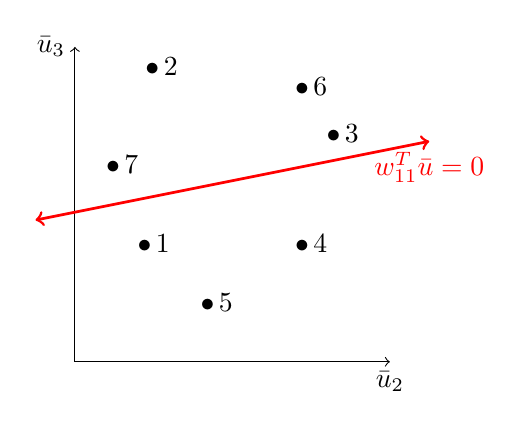
\begin{tikzpicture}
						
						\draw[->] (0,0) -- (4,0) node[anchor=north] {$\bar{u}_2$};
						\draw[->] (0,0) -- (0,4) node[anchor=east] {$\bar{u}_3$};
						\draw (1,1.5) node {$\bullet\,1$}; %label
						\draw (0.6,2.5) node {$\bullet\,7$}; %label
						\draw (1.8,0.75) node {$\bullet\,5$}; %label
						\draw (1.1,3.75) node {$\bullet\,2$}; %label
						\draw (3.4,2.9) node {$\bullet\,3$}; %label
						\draw (3,1.5) node {$\bullet\,4$}; %label
						\draw (3,3.5) node {$\bullet\,6$}; %label
						\draw[line width=1pt, red, <->] (-0.5,1.8) -- (4.5,2.8) node[anchor=north] {$w_{11}^T\bar{u} = 0$};
			\end{tikzpicture}}}
			\caption{Dividing a set of point to two equal subsets.}
			\label{fig:divideandconqueraduplicate}
		\end{subfigure}
		\begin{subfigure}[b]{0.45\textwidth}
			\centerline{\scalebox{0.85}{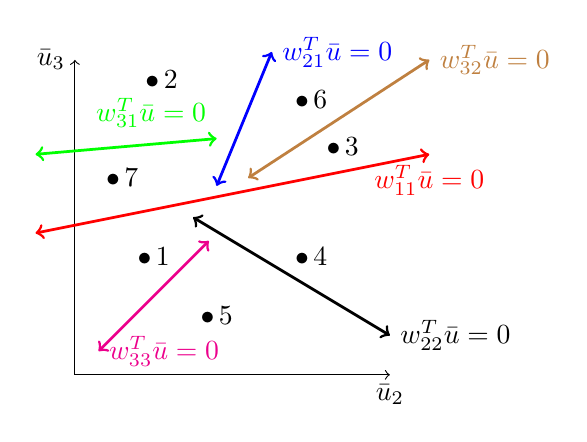
\begin{tikzpicture}
						
						\draw[->] (0,0) -- (4,0) node[anchor=north] {$\bar{u}_2$};
						\draw[->] (0,0) -- (0,4) node[anchor=east] {$\bar{u}_3$};
						\draw (1,1.5) node {$\bullet\,1$}; %label
						\draw (0.6,2.5) node {$\bullet\,7$}; %label
						\draw (1.8,0.75) node {$\bullet\,5$}; %label
						\draw (1.1,3.75) node {$\bullet\,2$}; %label
						\draw (3.4,2.9) node {$\bullet\,3$}; %label
						\draw (3,1.5) node {$\bullet\,4$}; %label
						\draw (3,3.5) node {$\bullet\,6$}; %label
						\draw[line width=1pt, red, <->] (-0.5,1.8) -- (4.5,2.8) node[anchor=north] {$w_{11}^T\bar{u} = 0$};
						\draw[line width=1pt, blue, <->] (1.8,2.4) -- (2.5,4.1) node[anchor=west] {$w_{21}^T\bar{u} = 0$};
						\draw[line width=1pt, brown, <->] (2.2,2.5) -- (4.5,4) node[anchor=west] {$w_{32}^T\bar{u} = 0$};
						\draw[line width=1pt, black, <->] (1.5,2) -- (4,0.5) node[anchor=west] {$w_{22}^T\bar{u} = 0$};
						\draw[line width=1pt, magenta, <->] (1.7,1.7) -- (0.3,0.3) node[anchor=west] {$w_{33}^T\bar{u} = 0$};
						\draw[line width=1pt, green, <->] (-0.5,2.8) -- (1.8,3) node[anchor=south east] {$w_{31}^T\bar{u} = 0$};
			\end{tikzpicture}}}
			\caption{Continued divisions until reaching singletons.}
			\label{fig:divideandconquerbduplicate}
	\end{subfigure}}
	\caption{The divide and conquer strategy. This figure is a duplicate of Fig. \ref{fig:divideandconquer} in order to make the proof easier to follow.}
	\label{fig:divideandconquerduplicate}
\end{figure}

Once an even division or separation is achieved, the next step is to design what we call a ``switching network''. Switching networks are small two-layer neural networks that can be parametrized by any number of points greater than $1$. Let $0_q$ denote the $q$-dimensional all-zero column vector. Roughly speaking, for the scenario in Fig. \ref{fig:divideandconqueraduplicate}, the corresponding switching network maps the input $\bar{u}\in\mathbb{R}^3$ to $[\begin{smallmatrix} \bar{u} \\ 0_3 \end{smallmatrix}]\in\mathbb{R}^6$ if $\bar{u}$ remains ``above'' the line $w_{11}^T \bar{u} = 0$, and to $[\begin{smallmatrix} 0_3 \\ \bar{u} \end{smallmatrix}]$ if  $\bar{u}$ remains ``below'' the line.\footnote{More precisely, there will be a small margin around the separating hyperplane where the aforementioned input-output relationships may fail. It turns out that this technical complication poses no issues for the patterns that we wish to memorize, as the margin can be made arbitrarily small.} We can now feed the first $3$ components of the output of the switch to one subnetwork, and the last $3$ components to another subnetwork. The two subnetworks are disconnected except that they share different components of the same output as inputs. The first subnetwork follows the same divide and conquer strategy with a switch, but only for the four points that remain over the line $w_{11}^T \bar{u} = 0$. 
The second subnetwork similarly processes the three points that remain under the line $w_{11}^T \bar{u} = 0$. The goal of the all-zero outputs is to deactivate one subnetwork when it is no longer relevant to process a given input. Subnetworks have ``subsubnetworks'' and so on until one arrives at a singleton dataset sample at each partition, as shown in Fig. \ref{fig:divideandconquerbduplicate}. 

Before proceeding to the next step, we formalize the constructions in Step 2 via the following lemma. 
%Due to space limitations, the proof of the lemma is provided in Appendix \ref{sec:switchinglemmaproof} of the supplemental material.
\begin{lemma}
\label{lemma:switch}
For $m \geq 2$, let $a_1,\ldots,a_m\in\mathbb{R}^{q}$ be distinct input patters whose first components equal $1$.

\begin{enumerate}[label={[\roman*]}]
\item There exists $w\in\mathbb{R}^{q}$, such that 
\begin{align}
\label{eq:wcond1} |\{i:w^Ta_i < 0\}| & = \lceil \tfrac{m}{2} \rceil, \\
\label{eq:wcond2} |\{i:w^Ta_i > 0\}| & = m-\lceil \tfrac{m}{2} \rceil.
\end{align}
\item Suppose further that the components of $a_i$s are all non-negative. Let $w\in\mathbb{R}^{q}$  satisfy (\ref{eq:wcond1}) and (\ref{eq:wcond2}). Let $0_q$ represent the $q$-dimensional all-zero vector. There is a two-layer network $\mathbf{S}:\mathbb{R}^q \rightarrow \mathbb{R}^{2q}$ 
that  satisfies the input-output relationships
\begin{align}
\label{eq:saicond}
\mathbf{S}(a_i) = \left\{\begin{array}{rl} \biggl[\begin{matrix} a_i \\ 0_q  \end{matrix}\biggr],  & w^Ta_i < 0,  \\ \vphantom{\scalebox{2.1}{$\int$}} \biggl[\begin{matrix} 0_q \\ a_i \end{matrix}\biggr],  & w^Ta_i > 0. \end{array} \right.,\,i=1,\ldots,m.
\end{align}
The network has $2q+2$ neurons. Two of the $2q+2$ neurons have $q$ weights, and the remaining $2q$ neurons have $2$ weights.
\end{enumerate}
\end{lemma}
\begin{proof}
Let us first prove [i]. Let $\bar{a}_{i} = [a_{i,2},\ldots,a_{i,q}]^T$ denote the $(q-1)$-dimensional vector consisting of all but the first component of $a_i$ (which equals $1$). First, we show the existence of $\bar{w}\in\mathbb{R}^{q-1}$ such that $\bar{w}^T \bar{a}_i \neq \bar{w}^T \bar{a}_j,\,\forall i \neq j$, or equivalently 
\begin{align}
\label{desiredwproperty} \bar{w}^T(\bar{a}_i - \bar{a}_j) \neq 0,\,\forall i \neq j. 
\end{align}
Since the input patterns $a_i$s are distinct, so are $\bar{a}_i$s, and thus $\bar{a}_i - \bar{a}_j$ are non-zero vectors. It follows that any unit norm $\bar{w}$ sampled uniformly at random on $\{x\in\mathbb{R}^q:\|x\|=1\}$ satisfies (\ref{desiredwproperty}) with probability $1$. Let us now order the resulting $(\bar{w}^T\bar{a}_i)$s in ascending order as
\begin{align}
\bar{w}^T\bar{a}_{i_1} < \cdots < \bar{w}^T\bar{a}_{i_{\lceil \frac{m}{2} \rceil}} < \bar{w}^T\bar{a}_{i_{\lceil \frac{m}{2} \rceil+1}} < \cdots < \bar{w}^T\bar{a}_{i_{m}},
\end{align}
for some permutation $i_1,\ldots,i_m$ of $1,\ldots,m$. We can now tune the bias as
\begin{align}
\bar{\bar{w}} \triangleq  - \frac{1}{2}\left(\bar{w}^T\bar{a}_{i_{\lceil \frac{m}{2} \rceil}} + \bar{w}^T\bar{a}_{i_{\lceil \frac{m}{2} \rceil+1}}\right).
\end{align}
The effect of the bias is the ordering (note the zero in the middle)
\begin{align}
\bar{\bar{w}} +\bar{w}^T\bar{a}_{i_1} < \cdots < \bar{\bar{w}} +\bar{w}^T\bar{a}_{i_{\lceil \frac{m}{2} \rceil}} < 0 < \bar{\bar{w}} +\bar{w}^T\bar{a}_{i_{\lceil \frac{m}{2} \rceil+1}} < \cdots < \bar{\bar{w}} +\bar{w}^T\bar{a}_{i_{m}}.
\end{align}
Therefore, the choice $w = [\begin{smallmatrix} \bar{\bar{w}} \\ {\bar{w}} \end{smallmatrix}]$ satisfies  conditions (\ref{eq:wcond1}) and (\ref{eq:wcond2}). This concludes the proof of [i]. 

We now prove [ii]. Let 
\begin{align}
C_1 & \triangleq 1+\max_{i\in\{1,\ldots,m\}}\max_{j\in\{1,\ldots,q\}} |a_{ij}|, \\
C_2 & \triangleq \min_{i\in\{1,\ldots,m\}} |w^Ta_{i}|.
\end{align}
Let $v =[v_1 \cdots v_{q}]^T\in \mathbb{R}^q$ represent an input to the neural network $\mathbf{S}$ that we shall construct. Also, let $v^+ = [v_1^+ \cdots v_{q}^+]^T$ and $v^-=[v_1^- \cdots v_{q}^-]^T \in \mathbb{R}^{q}$ denote the first and the last $q$ components of the $2q$-dimensional output of $\mathbf{S}$. We thus have $\mathbf{S}(v) = [\begin{smallmatrix} v^+ \\ v^- \end{smallmatrix}]$, and set
\begin{align}
v_j^+ & = \relu\Biggl( \biggr[\begin{matrix} v_j \\ \vphantom{\scalebox{1.3}{$\int$}} y^+ \end{matrix} \biggl]^T\biggr[\begin{matrix} 1 \\ \vphantom{\scalebox{1.3}{$\int$}} -\!\frac{C_1}{C_2} \end{matrix} \biggl] \Biggr),\,v_j^- = \relu\Biggl( \biggr[\begin{matrix} v_j  \\ \vphantom{\scalebox{1.3}{$\int$}} y^- \end{matrix} \biggl]^T\biggr[\begin{matrix} 1 \\ \vphantom{\scalebox{1.3}{$\int$}} -\!\frac{C_1}{C_2} \end{matrix} \biggl] \Biggr),\,j\in\{1,\ldots,q\},
\end{align}
where $y^+ = \relu(w^T v)$ and $y^- = \relu(-w^T v)$. Let us now verify (\ref{eq:saicond}). Consider some index $i$ with $w^T a_i < 0$, and suppose $v = a_i$. For any $j\in\{1,\ldots,q\}$, we have 
\begin{align}
v_j^+ & = \phi(v_j - \tfrac{C_1}{C_2}y^+)  = \phi(v_j) = \phi(a_{ij}) = a_{ij}.
\end{align}
The last equality holds as the components of $a_i$ are assumed to be all non-negative. Also, 
\begin{align}
v_j^-  = \phi(v_j - \tfrac{C_1}{C_2}y^-) 
= \phi(a_{ij} - \tfrac{C_1}{C_2}|w^Ta_i|)  \leq \phi(a_{ij} - C_1)  = 0.
\end{align}
Inequality follows as $\frac{|w^Ta_i|}{C_2} \geq 1$ and $\relu$ is monotonic. Since $v_j^- \geq 0$ obviously holds, we have $v_j^- = 0$. This proves the case $w^Ta_i < 0$ in (\ref{eq:saicond}). The remaining case  $w^Ta_i > 0$ can be verified in a similar manner. This concludes the proof of [ii], and thus that of Lemma \ref{lemma:switch} as well.
\end{proof}






\begin{figure}[h]
	\centerline{\scalebox{1}{\begin{tikzpicture}[
	arrowstyle/.style={decoration={markings,mark=at position 1 with
		{\arrow[scale=1.7,>=stealth]{>}}},postaction={decorate}},
roundnode/.style={circle, draw=blue!60, fill=blue!5, very thick, minimum size=2mm},
squarednode/.style={rectangle, draw=green!60, fill=yellow!5, very thick, minimum size=5mm},
squarednode2/.style={rectangle, draw=magenta!60, fill=magenta!5, very thick, minimum size=5mm},
squarednode3/.style={rectangle, draw=blue!60, fill=blue!5, very thick, minimum size=5mm},
squarednode4/.style={rectangle, draw=red!60, fill=red!5, very thick, minimum size=5mm},squarednode5/.style={rectangle, draw=orange!90, fill=orange!15, very thick, minimum size=5mm},]

\node[inner sep=0pt, minimum size=3mm](n1x) at (-0.75,-0.5){$=[\begin{smallmatrix} 1 \\ x_6 \end{smallmatrix}]$};

\node[inner sep=2pt, minimum size=3mm](n1) at (-1,0) {$u=\bar{x}_6$};
\node[squarednode](t) at (0.5,0) {$\mathbf{T}$};
\draw [arrowstyle](n1)--(t);
\node[squarednode2](s11) at (2.5,0) {$\mathbf{S}_{11}$};
\draw [arrowstyle](t)--node [below] {$\bar{u}=\bar{\bar{x}}_6$}(s11);
\node[squarednode2](s21) at (4,1.8) {$\mathbf{S}_{21}$};
\node[squarednode2](s22) at (4,-1.8) {$\mathbf{S}_{22}$};
\draw [arrowstyle](s11)--node [below] {$\,\,\bar{\bar{x}}_6$}(s21);
\draw [arrowstyle](s11)--node [below] {$0$}(s22);
\node[squarednode2](s32) at (5.5,0.9) {$\mathbf{S}_{32}$};
\node[squarednode2](s31) at (5.5,2.7) {$\mathbf{S}_{31}$};
\node[squarednode2](s33) at (5.5,-2.7) {$\mathbf{S}_{33}$};

\draw [arrowstyle](s21)--node [below] {$0$}(s31);
\draw [arrowstyle](s21)--node [below] {$\!\!\bar{\bar{x}}_6$}(s32);
\draw [arrowstyle](s22)--node [below] {$0$}(s33);

\node[squarednode3](g2) at (7,3.15) {$\gamma_2$};
\node[squarednode3](g7) at (7,2.25) {$\gamma_7$};
\node[squarednode3](g6) at (7,1.35) {$\gamma_6$};
\node[squarednode3](g3) at (7,0.45) {$\gamma_3$};
\node[squarednode3](g5) at (7,-3.15) {$\gamma_5$};
\node[squarednode3](g1) at (7,-2.25) {$\gamma_1$};
\node[squarednode3](g4) at (7,-0.9) {$\gamma_4$};

\draw [arrowstyle](s31)--node [above] {$0$}(g2);
\draw [arrowstyle](s31)--node [below] {$0$}(g7);
\draw [arrowstyle](s32)--node [above] {$\bar{\bar{x}}_6$}(g6);
\draw [arrowstyle](s32)--node [below] {$0$}(g3);
\draw [arrowstyle](s22)--node [above] {$0$}(g4);
\draw [arrowstyle](s33)--node [above] {$0$}(g1);
\draw [arrowstyle](s33)--node [below] {$0$}(g5);

%				\node[squarednode5](s32sum) at (8.5,0.9) {$\sum$};
%				\node[squarednode5](s31sum) at (8.5,2.7) {$\sum$};
%				\node[squarednode5](s33sum) at (8.5,-2.7) {$\sum$};
%				\node[squarednode5](s21sum) at (9.5,1.8) {$\sum$};
%				\node[squarednode5](s22sum) at (9.5,-1.8) {$\sum$};
\node[squarednode5](finalsum) at (9.5,0) {$\sum$};
\node[inner sep=2pt, minimum size=4mm](output) at (10.5,0) {$d_6$};
\draw [arrowstyle](finalsum)--(output); 

\draw [arrowstyle](g2)--node [above] {$0$}(finalsum);
\draw [arrowstyle](g7)--node [above] {$0$}(finalsum);
\draw [arrowstyle](g6)--node [above] {$d_6$}(finalsum);
\draw [arrowstyle](g3)--node [above] {$0$}(finalsum);
\draw [arrowstyle](g4)--node [above] {$0$}(finalsum);
\draw [arrowstyle](g1)--node [above] {$0$}(finalsum);
\draw [arrowstyle](g5)--node [above] {$0$}(finalsum);

%				\draw [arrowstyle](s33sum)--node [below] {$0$}(s22sum);
%				\draw [arrowstyle](s32sum)--node [below] {$d_6$}(s21sum);
%				\draw [arrowstyle](s31sum)--node [below] {$0$}(s21sum);
%				\draw [arrowstyle](s21sum)--node [below] {$d_6$}(finalsum);
%				\draw [arrowstyle](s22sum)--node [below] {$0$}(finalsum);
%				

	\end{tikzpicture}}}
	\caption{An example network architecture for the achievability result. The block $\mathbf{T}$ represents the transformation in Step 1. Blocks $\mathbf{S}_{ij}$ are the routing switches. Blocks $\gamma_i$ represent ReLU neurons with weights $\gamma_i$, and the $\sum$ block represents a ReLU neuron with all-one weights. This figure is a duplicate of Fig. \ref{fig:nnforachievability} in order to make the proof easier to follow.}
	\label{fig:nnforachievabilityduplicate}
\end{figure}



{\bf Step-3: } We can now proceed to describe the full network architecture, as shown in Fig. \ref{fig:nnforachievabilityduplicate} for the example in Step 2. The first layer of the network is an additive translation by the vector $[0\,M\cdots M]^T$, and is explained in Step 1 above. We use the notation $\mathbf{T}$ to denote the translation, which is followed by a sequence of switches as described in Step 2. In particular, $\mathbf{S}_{ij}$ provides the outputs of $\bar{u}$ and $0_3$ to its top and bottom branches, respectively, if its input $\bar{u}$ remains above the line defined by $w_{ij}$ in Fig. \ref{fig:divideandconquerbduplicate}.
By construction, the neurons on a given path of switches is activated for a unique dataset member. For example, the path $\mathbf{S}_{11},\mathbf{S}_{21},\mathbf{S}_{32}$ is activated only for the dataset member $x_6$. The path of switches that correspond to some $x_i$ is followed by a ReLU neuron whose weights satisfy the property that $\relu(\gamma_i^T \bar{\bar{x}}_i) = d_i$, where $\bar{\bar{x}}_i$ is the output of the first layer when the input to the network is $\bar{x}_i$. Since the first component of $\bar{\bar{x}}_i$ equals $1$ for any $i$, one can simply set the first component of $\gamma_i$ to be equal to $d_i$, and the rest of the component of $\gamma_i$ to be equal to zero. The final layers of the network simply adds all the outputs from the $\gamma_i$-neurons.


%are a cascade of ReLU neurons that simply add up all the outputs from the $\gamma_i$-neurons in a divide-and-conquer manner. We avoid summing up all the outputs of $\gamma_i$-neurons at once to achieve bounded number of weights for every neuron of the network. The topology of the summation neurons exactly mirrors the topology of switches.



In the figure, we also show the induced signals on the branches when the input is $u=\bar{x}_6$ as an example. Note that only the block $\mathbf{T}$, switches $\mathbf{S}_{11},\mathbf{S}_{21},\mathbf{S}_{32}$, the neuron with weight $\gamma_6^T$, and the a subset of the summation neurons remains active. Most of the neurons of the network are deactivated through zero signals. We also note that the desired output signal $d_6$ is obtained. 

%It is easily observed that all other desired input-output relationships are also satisfied. 

%Also, each subsequent summation unit will consist of $r$ sub-summation units operating on individual components. 

The construction generalizes to an arbitrary dataset of cardinality $n$ in the same manner. The only difference is that, in order to support  $r$-dimensional desired outputs as stated in the theorem, we need to use $r$ ReLU units in place of each $\gamma_i$ to reproduce the $r$ components of the desired output, as opposed to a single ReLU unit in the example above. Also, the final summation unit will consist of $r$ sub-summation units operating on individual components. Formally, the first layer for the general case is the translation $\mathbf{T}$ as before. Next, $\lceil \log_2 n \rceil$ layers of switches arranged on a binary tree structure act on the translated inputs, forming $n$ leaves as the output, where each leaf has the same dimension as the input. Let $h_1,\ldots,h_n$ denote the feature vectors produced at the leaf nodes after the switches. By Lemma 1, and a rearrangement of indices, we can guarantee that for every $i$, if the network input is $\bar{x}_i$, then $h_i = \bar{\bar{x}}_i$ and $h_j = 0,\,\forall j \neq i$. Here,  $\bar{\bar{x}}_i = \mathbf{T}([1\,\, x_i^T]^T)$, as defined in Fig. \ref{fig:nnforachievabilityduplicate}. Each leaf is then followed by a single-layer network that can map $\bar{\bar{x}}_i$ to its corresponding desired output vector $d_i$. Specifically, there exists $U_i$ such that $d_i = \phi(U_i \bar{\bar{x}}_i)$. Indeed, since $\sum_k u_{i,j,k}\bar{\bar{x}}_{i,k} = d_{i,j}$ has to be satisfied, one can pick $u_{i,j,k}=0,\,k\neq 1$ and $u_{i,j,1} = d_{i,j}/\bar{\bar{x}}_{i,1} = d_{i,j}$, where the last equality holds as $\bar{\bar{x}}_{i,1}=1$ by construction. The overall network output is the accumulation of the outputs of the $U_i$-neurons, and is given by $f(\overline{x}_i) = \phi(\sum_{i=1}^n \phi(U_ih_i))$. Let us show that all input-output relationships are satisfied so that the claim $f(\bar{x}_i) = d_i,\,\forall i$ in the statement of the theorem holds. If the input is $\bar{x}_i$, we have $h_i = \bar{\bar{x}}_i$ and $h_j = 0,\,j\neq i$, by construction. As a result, $f(\overline{x}_i) = \phi(\phi(U_i \bar{\bar{x}}_i)) = \phi(d_i) = d_i$, as desired. The last equality holds as the components of $d_i$ are assumed non-zero in the statement of the theorem (A ReLU network cannot provide a negative output.).

Let us now calculate the number of active neurons and weights when the input belongs to any member of the dataset. The block $\mathbf{T}$ always remains active and consists of $q-1$ neurons with weight $2$. There are at most $\lceil \log_2 n \rceil$ active switches per input. Each switch contains $2q+2$ neurons with $6q$ weights total. There is one active block $\gamma_i$ consisting of $r$ neurons with $q$ weights each. Finally, the sum unit has $r$ active weights. Hence, an upper bound on the total number of active neurons are given by 
\begin{align}
q-1  + (2q+2)\lceil \log_2 n \rceil+r+1 & = 2(q+1)\lceil \log_2 n \rceil + q+r\\
& \in O(r+q\log n),
\end{align}
and an upper bound on the number of active weights can be calculated to be 
\begin{align}
2(q-1) + 6q(2q+2)\lceil \log_2 n \rceil + rq+r & =12q(q+1)\lceil \log_2 n \rceil + (r+2)q+r-2 \\
& \in O(rq+q^2\log n).
\end{align}
 This concludes the proof of the theorem.

%q-1  + (2q+2)\lceil \log_2 n \rceil+r+1$

%2(q-1) + 6q(2q+2)\lceil \log_2 n \rceil + rq+r$

%%
%\section{Proof of	 Lemma \ref{lemma:switch}}
%\label{sec:switchinglemmaproof}


%\section{Proof of Lemma \ref{lemma:treeleafnodecounterlemma}}
%\label{sec:proofoftreeleafnodecounterlemma}
%We use the notation $a \in b$ to indicate that $a$ is a children of $b$. 
%Consider an arbitrary path $\nu_0\rightarrow \nu_1 \rightarrow \cdots \rightarrow \nu_{L}$. We have $\prod_{\ell=1}^L \sigma(\nu_{\ell}) \leq K$. Let $\chi(\nu_{L-1})$ denote the number of children of $\nu_{L-1}$. Summing up over all children of $\nu_{L-1}$, we have
%\begin{align}
%\prod_{\ell=1}^{L-1}\sigma(\nu_{\ell})  \sum_{\nu_{L} \in \nu_{L-1}} \sigma(\nu_{L}) \leq K \chi(\nu_{L-1})
%\end{align}
%Since $\chi(\nu_{L-1}) = \sigma(\nu_{L})$ for every $\nu_{L} \in \nu_{L-1}$, we obtain
%\begin{align}
%\prod_{\ell=1}^{L-1}\sigma(\nu_{\ell})  \Biggl(\sum_{\nu_{L} \in \nu_{L-1}} 1 \Biggr) \leq K 
%\end{align}
%Continuing in the same manner by summing over all children of $\nu_{\ell}$ and then simplifying by using the identity $\chi(\nu_{\ell-1}) = \sigma(\nu_{\ell})$ for $\ell=L-2,\ldots,1$, we arrive at
% \begin{align}
%\sum_{\nu_{1} \in \nu_{0}} \cdots \sum_{\nu_{L} \in \nu_{L-1}} 1 \leq K.
% \end{align}
% The left side is merely the number of leaf nodes. This concludes the proof of the lemma.

%\section{Proofs of Main Results for Threshold Networks}
%\label{sec:proofofthresholdtheorems}
%\subsection{Proof of Theorem \ref{th:thresholdach}}
%\label{sec:proofoftheoremthresholdach}
%As identified by several studies, and also by  \citet{rajput2021exponential} in particular, a key challenge in threshold networks is that the amplitude information of the input patterns is lost as soon as one passes through the first layer of the network. This is why we need a mapping that maps each input pattern to a unique binary representation in the first layer. The existence of such a mapping has been elegantly proven in \citet[Section 5, Step 1]{rajput2021exponential} by using the idea of random Gaussian weights. Their argument reveals that there exists a layer with $\smash{O(\frac{\log n}{\delta})}$ neurons that can map each input pattern to a unique binary representation. This layer becomes the first layer of our network. The rest of the layers of the network is exactly the same as in Steps 2 and 3 of the proof of Theorem \ref{th:reluach} in Appendix \ref{sec:reluachthproofer}, with the only exception being that all ReLU activation functions are replaced by threshold activation functions. Remarkably, when its inputs is a binary vector, the functionality of the switching network as constructed in the proof of Lemma \ref{lemma:switch} can easily be verified to remain the same under such a change in activation functions. Likewise, the functionality of the summation units will remain the same, given that they will only admit either two zeros or a zero and one as inputs, when the input pattern corresponds to a dataset pattern. As a result, we obtain the same bound in Theorem \ref{th:reluach} for the special case $\smash{p=\frac{\log n}{\delta}}$ in the statement of Theorem \ref{th:reluach}. This concludes the proof of Theorem \ref{th:thresholdach}.
%\subsection{Proof of Theorem \ref{th:thresholdconv}}
%\label{sec:proofoftheoremthresholdconv}
% For a threshold network, the configuration tree corresponding to the network and the dataset can be constructed in the same manner as described in the proof of Theorem \ref{th:reluconv}. The difference is that for a threshold network, the output configurations at the leaves of the tree correspond to all possible outputs that the network can provide. Since there are at most $2^{\alpha}$ leaves and the desired output vectors are all distinct, we need $n \leq 2^{\alpha}$ for successful memorization. Taking the logarithms of both sides of the inequality concludes the proof of the theorem.
%

